\documentclass[landscape,usenames,dvipsnames]{sciposter}
\renewcommand{\papertype}{custom}
\renewcommand{\sectionsize}{\large}


% edit pointsize, width, height, and fontsize parameters as needed
% DO ensure that values in the \special commands match!
\usepackage[pass,paperwidth=43.6in,paperheight=24.5in]{geometry}
\renewcommand{\fontpointsize}{25pt}
\setmargins[2.5cm]

%\renewcommand{\subsectionsize}{\large \textcolor{\SectionCol}}
%\usepackage[spanish]{babel}
% or whatever
\usepackage{tikz}
\usetikzlibrary{arrows,automata,positioning}
\usepackage[latin1]{inputenc}
\usepackage{amsmath,amsthm,amssymb,bm}
\usepackage{multicol}
\usepackage{listings}
\usepackage{enumerate, wrapfig}
\usepackage{colortbl}
\usepackage[absolute]{textpos}
%\usepackage{subfigure}
\usepackage{caption}
\usepackage{graphicx}
\graphicspath{ {images/} }

%\newcommand{\reed}[1]{\relax}
%\newcommand{\abdullah}[1]{\relax}
%\newcommand{\tatum}[1]{\relax}
%\newcommand{\eric}[1]{\relax}
%\newcommand{\christian}[1]{\relax}
%\newcommand{\Fix}[1]{\relax}
\newcommand{\reed}[1]{{\color{magenta}\bfseries [#1]}}
\newcommand{\abdullah}[1]{{\color{blue}\bfseries [#1]}}
\newcommand{\tatum}[1]{{\color{orange}\bfseries [#1]}}
\newcommand{\eric}[1]{{\color{green}\bfseries [#1]}}
\newcommand{\christian}[1]{{\color{cyan}\bfseries [#1]}}
\newcommand{\Fix}[1]{{\color{red}\bfseries [#1]}}
\newcommand{\Comment}[1]{}
\newcommand{\Space}[1]{}
\newcommand{\Num}[1]{#1}

\newcommand{\term}[1]{\emph{\textbf{#1}}}

\newcommand{\R}{\mathbb{R}}
\newcommand{\Q}{\mathbb{Q}}
\newcommand{\Z}{\mathbb{Z}}
\newcommand{\N}{\mathbb{N}}

\theoremstyle{definition}
\newtheorem{definition}{Definition}[section]
\theoremstyle{remark}
\newtheorem{remark}[definition]{Remark}
\theoremstyle{remark}
\newtheorem{example}[definition]{Example}
\theoremstyle{plain}
\newtheorem{theorem}[definition]{Theorem}
\newtheorem{conjecture}[definition]{Conjecture}

\lstdefinelanguage{pecan}{
	keywords=[1]{forall, exists, max, min, sup, inf, are, is, if, then, match, with, case, end, let, be, in, else, iff},
	keywordstyle=[1]\color{blue}\bfseries,
	keywords=[2]{false, true, sometimes},
	commentstyle=\color{CadetBlue}\textit,
	stringstyle=\color{ForestGreen}, % string literal style
	keywordstyle=[2]\color{orange}\bfseries,
	keywords=[3]{assert_prop,Structure,defining,Theorem,Prove,Example,Alias,Restrict,Define,Display,Execute,load,shuffle,import,save_aut,save_aut_img,that,context,end_context,forget,shuffle,shuffle_or,using,of},
	keywordstyle=[3]\color{teal}\bfseries,
	keywords=[4]{@annotation,@postprocess,@no_simplify,@simplify,@simplify_states,@simplify_edges},
	keywordstyle=[4]\color{purple}\bfseries,
	literate=%
	    {\#}{{{\color{teal}\bfseries\#}}}1
	    {+}{{{\color{red}+~}}}1
	    {-}{{{\color{red}-~}}}1
        {:=}{{{\color{red}:=~}}}1
        {..}{{{\color{red}..~}}}1
        {\{}{{{\color{red}\{}}}1
        {\}}{{{\color{red}\}}}}1
        {|}{{{$\color{red} \lor~$}}}1
        {*}{{{\color{red}*~}}}1
        {:}{{{\color{red}:~}}}1
        {>}{{{\color{red}>~}}}1
        {<}{{{\color{red}<~}}}1
        {<=>}{{{$\color{red}\Leftrightarrow~$}}}1
        % <= conflicts with <=> as iff, so I commented it out because it's more importnat that <=> not look weird (it becomes \leq > with the following line).
        % But might as well keep something, so I keep \iff
        % {<=}{{{$\color{red} \leq$}}}1
        % Also got rid of >= for consistency.
        % {>=}{{{$\color{red} \geq$}}}1
        {.}{{{\color{red}.~}}}1
        {&}{{{$\color{red} \land~$}}}1
        {!}{{{$\color{red}\lnot~$}}}1
        {!=}{{{$\color{red} \neq$}}}1
        {=}{{{\color{red}=~}}}1
        {exists }{{{$\color{red}\exists$}}}1
        {forall }{{{$\color{red}\forall$}}}1,
    sensitive=false, % keywords are not case-sensitive
    morecomment=[l]{//}, % l is for line comment
    morecomment=[s]{/*}{*/}, % s is for start and end delimiter
    morestring=[b]", % defines that strings are enclosed in double quotes
    showstringspaces=false
}

\lstnewenvironment{pecan}
  {
    \lstset{
        language=pecan, 
        basicstyle=\small\ttfamily, 
        mathescape=true
        }
  }
  {
  }

\lstnewenvironment{pecan_output}
  {
    \lstset{
        basicstyle=\small\ttfamily,
        mathescape=true
        }
  }
  {
  }

\newcommand{\pecaninline}[1]{\lstinline[language=pecan,basicstyle=\small\ttfamily,mathescape]{#1}}


\newtheorem{thm}{Theorem}%[section] % uncomment [section] to number within section
\newtheorem*{thm*}{Theorem}
\newtheorem{lem}{Lemma}
\newtheorem{cor}[thm]{Corollary}
\newtheorem{prop}[thm]{Proposition}
\newtheorem{rem}[thm]{Remark}
\newtheorem{cond}[thm]{Condition}
\newtheorem*{namedtheorem}{Theorem}
\newtheorem*{ex}{Example}
\newtheorem*{defin}{Definition}
\newtheorem{env}[thm]{Variation}
\renewcommand {\theequation}{\arabic{section}.\arabic{equation}}

%Lines 54-73 define box theorem. You can do similar things to put boxes around conjectures, corollaries, ect, or use the mdframe to just create a box
\usepackage[framemethod=TikZ]{mdframed}
\definecolor{light-blue}{RGB}{197,219,249}
\mdfdefinestyle{MyFrame}{linecolor=light-blue,
    outerlinewidth=1.5pt,
    roundcorner=0pt,
    innertopmargin=7pt,
    innerbottommargin=7pt,
    innerrightmargin=15pt,
    innerleftmargin=15pt,
    backgroundcolor=light-blue}
\mdfdefinestyle{thmsytle}{linecolor=orange,
    outerlinewidth=2pt,
    roundcorner=20pt,
    innertopmargin=15pt,
    innerbottommargin=15pt,
    innerrightmargin=15pt,
    innerleftmargin=15pt,
    backgroundcolor=white,
	}


\mdtheorem[style=thmsytle]{MDtheorem}{Theorem}
\newcommand*{\Title}{}
\newenvironment{boxthm}[1][]{%
\refstepcounter{thm}
    \ifstrempty{#1}{\begin{MDtheorem}}%
    {\begin{MDtheorem}[(#1)]}
}{%
    \end{MDtheorem}%
}%

%%hyperlinks
\usepackage{hyperref}
 
% \usepackage[
% backend=biber,
% style=alphabetic,
% sorting=ynt
% ]{biblatex}

% \addbibresource{bibliography.bib}


%\definecolor{BoxCol}{rgb}{0.9,0.9,0.9}
% uncomment for grey background to \section boxes
% for use with default option boxedsections

\definecolor{BoxCol}{rgb}{.06,.16,.28}


\definecolor{SectionCol}{rgb}{1,1,1}

\definecolor{blue}{rgb}{0,0,1}
\definecolor{orange}{rgb}{.93,.29,0.1}
\definecolor{white}{rgb}{1,1,1}

\newtheorem{Features}{Features}

\title{Pecan: An Automated Theorem Prover}

\author{
Authors: Zhengyao Lin, Eric Ma, Reed Oei, Yikai Teng, Pavle Vuksanovic \\
Graduate Mentors: Christian Schulz, Mary-Angelica Tursi \\
Faculty Advisor: Philipp Hieronymi}

%\institute{University of Illinois at Urbana-Champaign}
%\email{}  shows author email address below institute

%\date is unused by the current \maketitle

%%%%%%%%%%%%%%%%%%%%%%%
% Logo for Poster
%%%%%%%%%%%%%%%%%%%%%

\leftlogo[.7]{igl-logo-small.png} % defines logo to left of title (with scale factor)
\rightlogo[.6]{imark.png} % same but on right

%%%%%%%%%%%%%%%%%%%
% Start of document
%%%%%%%%%%%%%%%%%%%
\begin{document}
%%%%%%%%%%%%%%%%%%%%%%
%% Poster Set up
%%%%%%%%%%%%%%%%%%%%%%%
% \conference{Undergraduate Research Symposium SP 2020}
\conference{2021 Joint Mathematics Meetings}

\maketitle
\vspace{-3ex}
\begin{multicols}{3}  % sets up 3 column poster



%%%%%%%%%%%%%%%%%%%%%%
%% Start of First Column
%%%%%%%%%%%%%%%%%%%%%%%
\section*{Introduction}
% \begin{mdframed}[style=MyFrame]
% \subsection*{Automated Theorem Proving}
% \end{mdframed}

\textbf{Pecan} is an automated theorem prover for reasoning about \emph{automatic sequences}, which are sequences that can be recognized by some (typically finite) automaton.
Automated theorem provers and automatic sequences have diverse applications: in computer science, they are commonly used for program verification; in mathematics, they have found uses in logic, number theory, and combinatorics. Pecan is capable of proving any statement expressed in terms of B\"uchi automata and first-order logic connectives.

We have used Pecan to prove many theorems about a special class of automatic sequences called \emph{Sturmian words}, and we are currently exploring extensions including deciding sentences involving linear inequalities with integer and quadratic irrational coefficients, and
visualization of fractals defined by B\"uchi automata.

%%%%%%%%%%%%%%%%%%%%%%%%%%%%%%%%%%%%%
%% Pecan
%%%%%%%%%%%%%%%%%%%%%%%%%%%%%%%%%%%%%
\section*{Overview}

Pecan programs are made up of \emph{predicates} and \emph{directives}:

\begin{itemize}
    \item predicates: defined either by loading automata defined in files, translating linear temporal logic formulas into B\"uchi automata, or some combination of these using first order logic and equality.
\begin{pecan}
y is successor_of(x) := x < y & forallz. z <= x | y <= z
\end{pecan}

    \item directives: commands to the Pecan interpreter, such as: \pecaninline{Theorem}, which asks Pecan to prove a theorem, or \pecaninline{save_aut}, which asks Pecan to build the automaton corresponding to some predicate and save it to a file
\begin{pecan}
Theorem ("Addition is commutative.", { forallx,y. x + y = y + x }).
\end{pecan}

\end{itemize}

You can try out Pecan online at \url{http://reedoei.com/pecan}.

% \section*{The Chicken McNugget Problem}

% % In the 1980s, Henri Picciotto asked the following problem in his algebra textbook:

% \begin{quote}
%     What is the greatest number of chicken nuggets that cannot be ordered using only boxes of 6, 9, and 20?
% \end{quote}

% We call all such numbers \textbf{non-purchasable}, and we can define them in Pecan as follows:

% \begin{lstlisting}[language=pecan, basicstyle=\normalsize\ttfamily, mathescape=true, frame=single]
% Restrict n,m,a,b,c are binary.
% n is purchasable := n is binary & existsa,b,c. n =$\ $6*a $\color{red} +$ 9*b $\color{red} +$ 20*c
% n is non_purchasable := n is binary & !(n is purchasable)
% \end{lstlisting}

% We can then define the largest non-purchasable number naturally as:
% \begin{lstlisting}[language=pecan, basicstyle=\normalsize\ttfamily, mathescape=true, frame=single]
% largest(n) := n is non_purchasable & 
%               forallm. if m is non_purchasable then n >= m
% \end{lstlisting}

% \begin{figure}
%     \centering
%     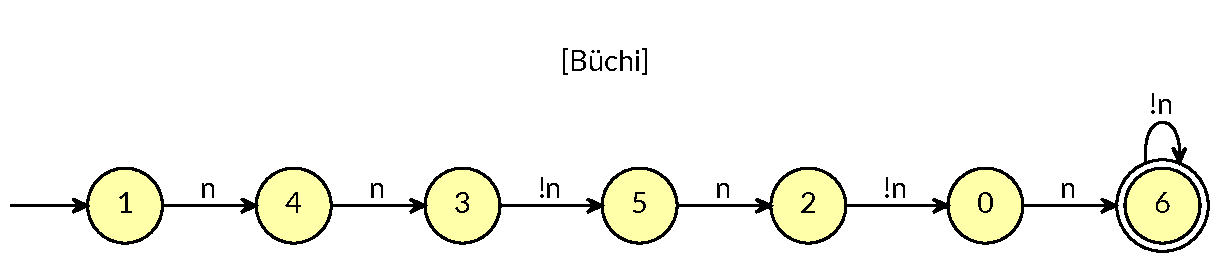
\includegraphics[width=\textwidth]{images/largest_not_purchasable.pdf}
%     \caption{The B\"uchi automaton representing \pecaninline{largest(n)}, which accepts $110101_2$ ($43$ in base 10) in least significant digit first representation.}
%     \label{fig:largest_non_purchasable}
% \end{figure}

% We can also ask Pecan to show us what numbers \pecaninline{largest} accepts, and it will automatically perform the necessary conversions.
% \begin{pecan}
% Example (natFormat, { largest(n) }). // Prints [(n,43)]
% \end{pecan}

% \section*{The Thue-Morse Word}

% We now turn to \textbf{automatic sequences}, words defined by automata, starting with the Thue-Morse word, $T$. 
% The $n$-th digit of the Thue-Morse word, $T[n]$, is $1$ if the binary representation of $n$ has an odd number of $1$'s, and $0$ otherwise.
% The Thue-Morse word starts with: $01101001100101101001011001101001\ldots$

% \begin{defin}
%     A word $w$ is a \textbf{square} if it is of the form $w = xx$ for some word $x$.
%     Similarly, $w$ is a \textbf{cube} if it is of the form $w = xxx$ for some word $x$.
% \end{defin}

% \begin{mdframed}[style=MyFrame]
% \begin{thm}
%     The Thue-Morse word does not contain any cubes.
% \end{thm}
% \end{mdframed}

% Below is a Pecan definition of cubes in the Thue-Morse word and the theorem we would like to prove.
% \begin{lstlisting}[language=pecan, basicstyle=\normalsize\ttfamily, mathescape=true, frame=single]
% Restrict i,j,n are binary.
% square(i, n) := n > 0 & T[i..i+n] = T[i+n..i+2*n]
% cube(i,n) := square(i, n) & square(i+n, n)
% Theorem ("T does not contain cubes", { !(existsi,n. cube(i,n)) }).
% \end{lstlisting}

% \begin{lstlisting}[basicstyle=\normalsize\ttfamily, mathescape=true, frame=single]
% [INFO] Checking if T does not contain cubes is true.
% $\color{ForestGreen} \text{T does not contain cubes is true.}$
% \end{lstlisting}

% \begin{mdframed}[style=MyFrame]
% \begin{thm}
% There are no overlapping squares, i.e., words of form $0x0x0$ or $1x1x1$ for some nonempty word $x$. 
% \end{thm}
% \end{mdframed}

% We can check it by running the following Pecan commands.

% \begin{lstlisting}[language=pecan, basicstyle=\normalsize\ttfamily, mathescape=true, frame=single]
% Theorem ("T does not contain overlapping squares.", 
%     { !(existsi,n. n > 0 & square(i,n) & T[i] = T[i+2*n]) }).
% \end{lstlisting}
% Pecan verifies the theorem: 
% \begin{lstlisting}[basicstyle=\normalsize\ttfamily, mathescape=true, frame=single]
% [INFO] Checking if T does not contain overlapping squares is true.
% $\color{ForestGreen} \text{T does not contain overlapping squares is true.}$
% \end{lstlisting}

%%%%%%%%%%%%%%%%%%%%%%%%%%%%%%%%%%%%%
%% New Section
%%%%%%%%%%%%%%%%%%%%%%%%%%%%%%%%%%%%%
\section*{Characteristic Sturmian Words}
A \emph{cutting sequence} for a curve is a sequence of $0$'s and $1$'s, corresponding to when the line crosses vertical and horizontal grid lines, respectively.
The \emph{characteristic Sturmian word with slope $\alpha$} is an infinite binary sequence defined by the cutting sequence of $y = \alpha x$ for some irrational $\alpha \in (0,1)$ in the Cartesian plane.
Figure~\ref{fig:fib_word} shows the beginning of the characteristic Sturmian word with slope $\frac{1}{\phi}$, which begins $0100101001\ldots$.

\centerline{
\begin{minipage}{.6\columnwidth}
\begin{figure}
	\centering
    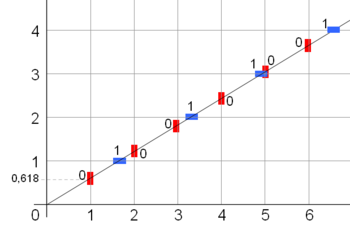
\includegraphics[width=0.8\columnwidth]{images/Fibonacci_word_cutting_sequence.png}
    \captionof{figure}{Characteristic Sturmian word with slope $\frac{1}{\phi}$}
    \label{fig:fib_word}
\end{figure}
\end{minipage}}

Sturmian words are automatic sequences: there are automata which calculate their $n$-th digit given the representation of $n$ in the appropriate numeration system.
For Sturmian words, we use a family of numeration systems called \emph{Ostrowski numeration systems}.
With the addition automaton for general Ostrowski numeration systems, we are able to use Pecan to \emph{automatically prove} properties about Sturmian words. 

\columnbreak

\section*{Theorems about Sturmian Words}

Sturmian words have many interesting properties that we can use Pecan to automatically prove:
one particularly fundamental result is that Sturmian words are not \emph{eventually periodic}.
\begin{mdframed}[style=MyFrame]
\begin{defin}
    A word is \emph{eventually periodic} if it is of the form $abbbbb \ldots$ for some subwords $a$ and $b$ (e.g., $0.1024545454545\ldots$ where the repeating part is $45$).
\end{defin}


\begin{thm*}
Sturmian words are not eventually periodic.
\end{thm*}

\begin{proof}
In Pecan, we can prove this theorem simply by writing the definition of ``eventually periodic'' and stating the theorem.
Running the Pecan program below proves the theorem.
\begin{pecan}
eventually_periodic(a, p) := 
    p > 0 & existsn. foralli. if i > n then C[i] = C[i+p]
    
Theorem ("Sturmian words are not eventually periodic", { 
    foralla,p. if p > 0 then !eventually_periodic(a,p) 
}).
\end{pecan}
We omit the pictures of the intermediate automata, as they have hundreds (or even thousands) of states, and so it is nearly impossible to understand them by looking at pictures of them.
\end{proof}
\end{mdframed}


In this example, we state and prove a theorem about \textbf{all} Sturmian words.
        \begin{itemize}
            \item Previous theorem provers (e.g., Walnut [2]) in the same area could only prove theorems about a single Sturmian word, or small subsets of Sturmian words
        \end{itemize}
        
Using Pecan, we proved many other theorems about Sturmian words, including many classical results, some recent results, and notably, some \textbf{new} results.
    \begin{itemize}
        \item Sturmian words are not eventually periodic.
        \item Sturmian words contain cubes.
        \item Sturmian words contain palindromes of every length.
        \item Sturmian words contain only finitely many antisquares and antipalindromes.
        \item Every subword of a Sturmian word occurs infinitely often.
        \item The unique special factor of length $n$ is the reverse of the length $n$ prefix of the Sturmian word.
        \item[$\vdots$]
    \end{itemize}

\section*{Multiplying Ostrowski Representations}

In the Ostrowski numeration systems mentioned previously, every natural number has a unique \emph{$\alpha$-Ostrowski representation}.

Specifically, for any irrational $\alpha$ with an infinite continued fraction expansion, there is a unique way to represent any natural number as a sum of products of the denominators of the consecutive continued fraction approximations of $\alpha$.

We implemented an extension to Pecan to construct an automaton recognizing order in the ring $\mathbb Z [ \alpha ]$ using $\alpha$-Ostrowski representations, where $\alpha$ is a quadratic irrational using a method developed by Hieronymi et al. [4]. 
Unfortunately, we found that the size of this automaton scaled quickly with the complexity of the continued fraction expansion of $\alpha$.

\begin{itemize}
    \item For $\alpha = 1/\phi = (\sqrt 5 - 1)/2$, with continued fraction expansion $[0;1,1,\dots]$, the automaton for recognition of order in $\mathbb Z [ \alpha ] $ had 2,134 states.
    
    \item For $\alpha = \sqrt 2 - 1$, with continued fraction expansion $[0;2,2,\dots]$, the automaton for recognition of order in $\mathbb Z [ \alpha ] $ had 218,072 states.
    
    \item For more complex $\alpha$, we were unable to compute the automata due to their large size.
\end{itemize}

\columnbreak

\section*{Fractals}

\emph{Automatic fractals} are fractals recognizable by an automaton, via some suitable mapping between words and reals. 
We developed an extension to Pecan that maps the set of words accepted by an automaton to a subset of $[0, 1]^n$, and used it to plot some fractals.

\begin{itemize}
    \item Automata and plot of the Cantor set and Cantor distance function:
\end{itemize}

\begin{center}
    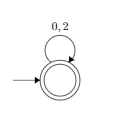
\includegraphics[width=5.2cm]{FA20/images/fractals/cantor-automata.png}
    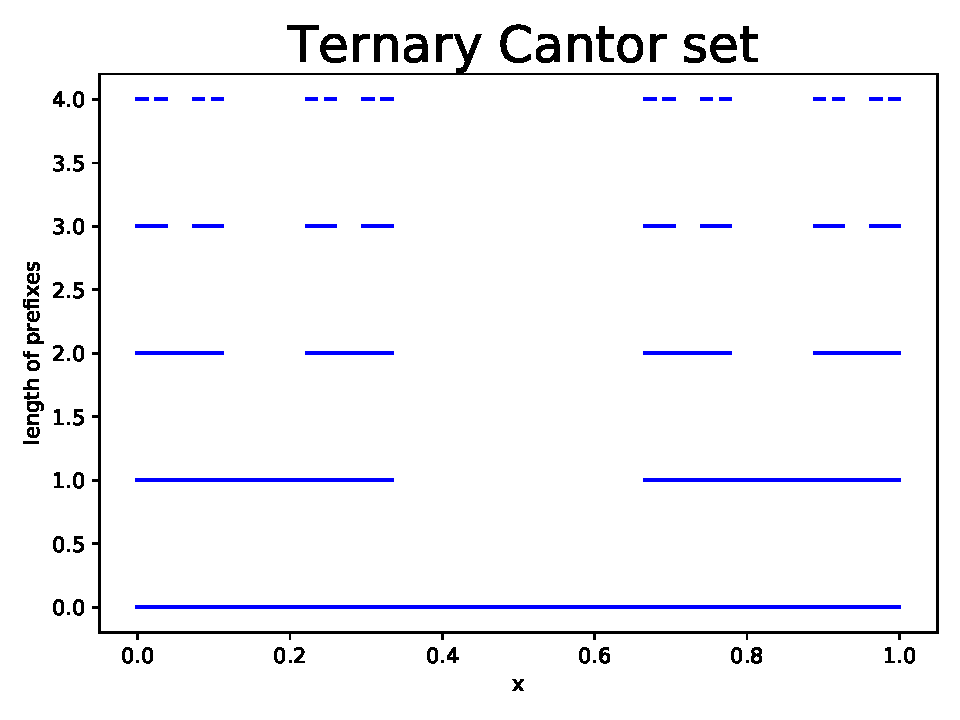
\includegraphics[width=7.8cm]{FA20/images/fractals/cantor3.pdf}
    \qquad
    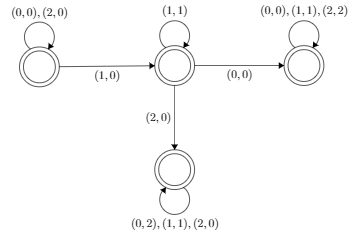
\includegraphics[width=7.8cm]{FA20/images/fractals/cantord-automata.png}
    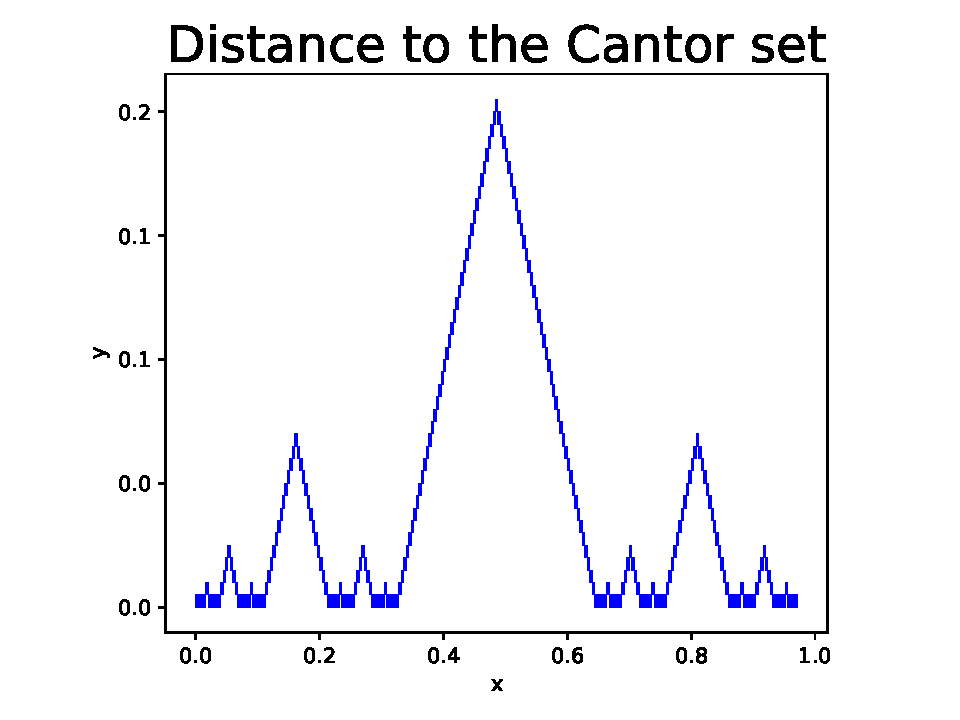
\includegraphics[width=7.8cm,height=5.2cm]{FA20/images/fractals/cantord.pdf}
\end{center}

{ \footnotesize The automaton for the distance function to the Cantor set comes from \cite{gorman2019continuous} }

\begin{itemize}
    \item Using a similar automata to the Cantor set, we have the following:
\end{itemize}
    
\begin{center}
    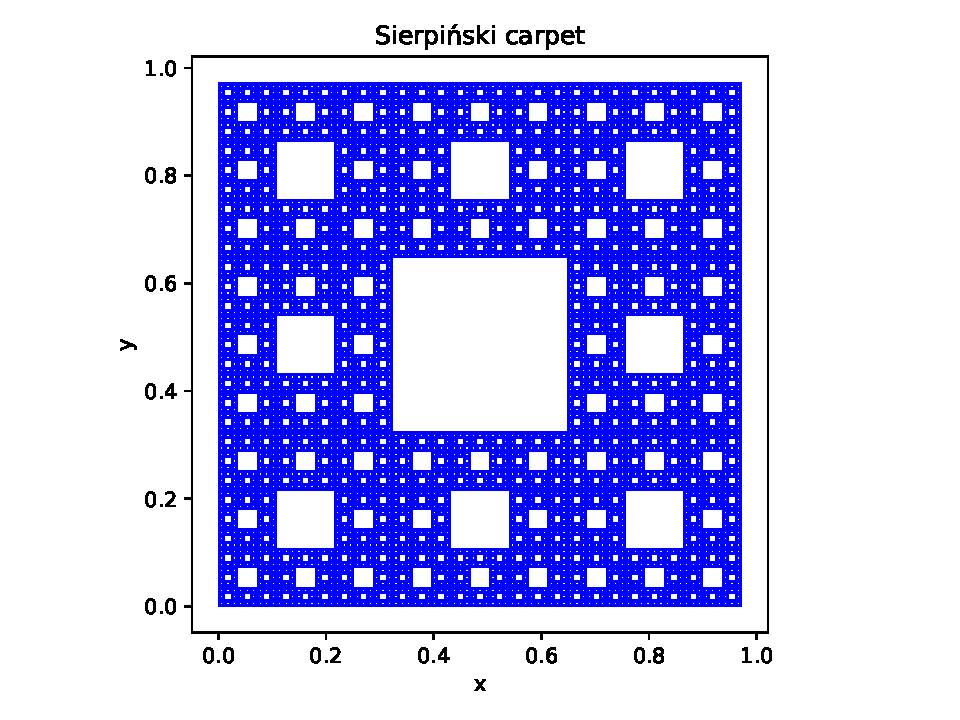
\includegraphics[width=9cm]{FA20/images/fractals/sierpinski-3-l5.pdf}
    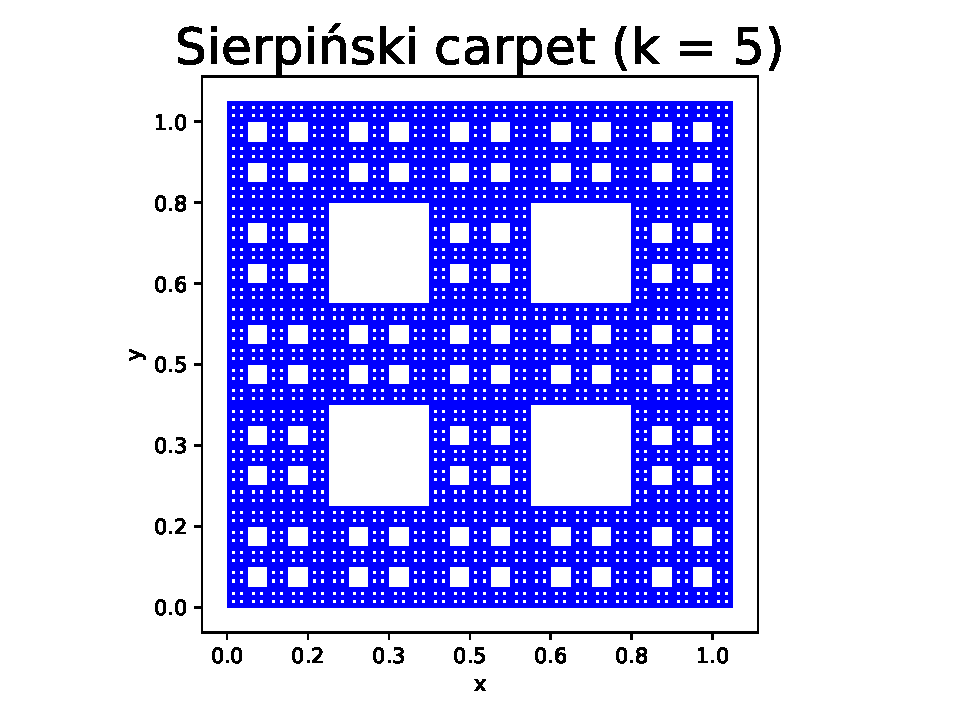
\includegraphics[width=9cm]{FA20/images/fractals/sierpinski-5-l3.pdf}
    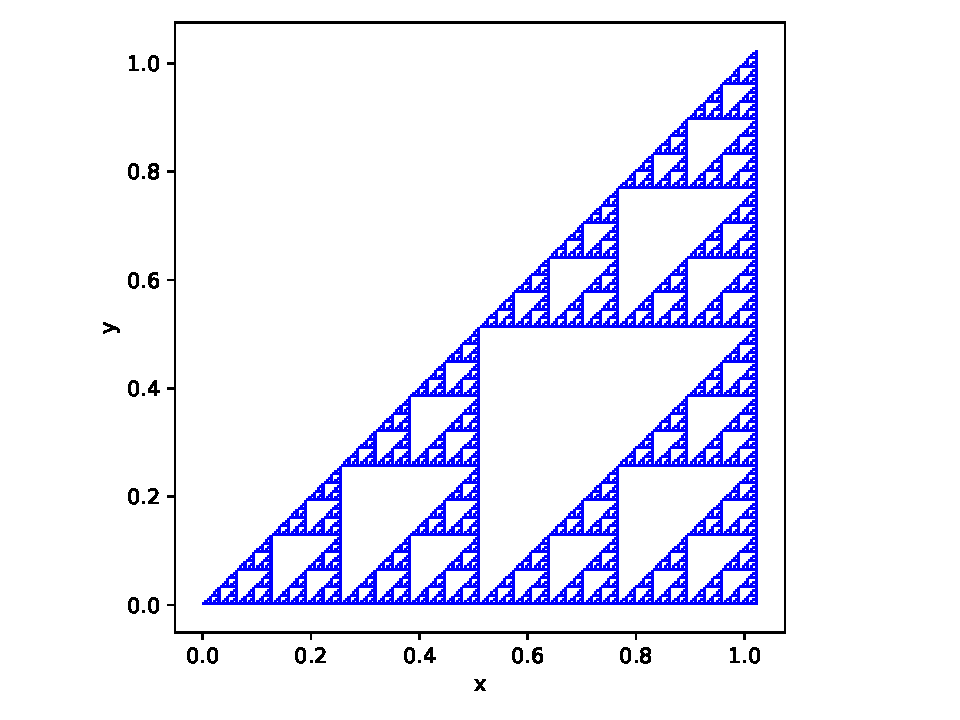
\includegraphics[width=9cm]{FA20/images/fractals/pascal2.pdf} \\
    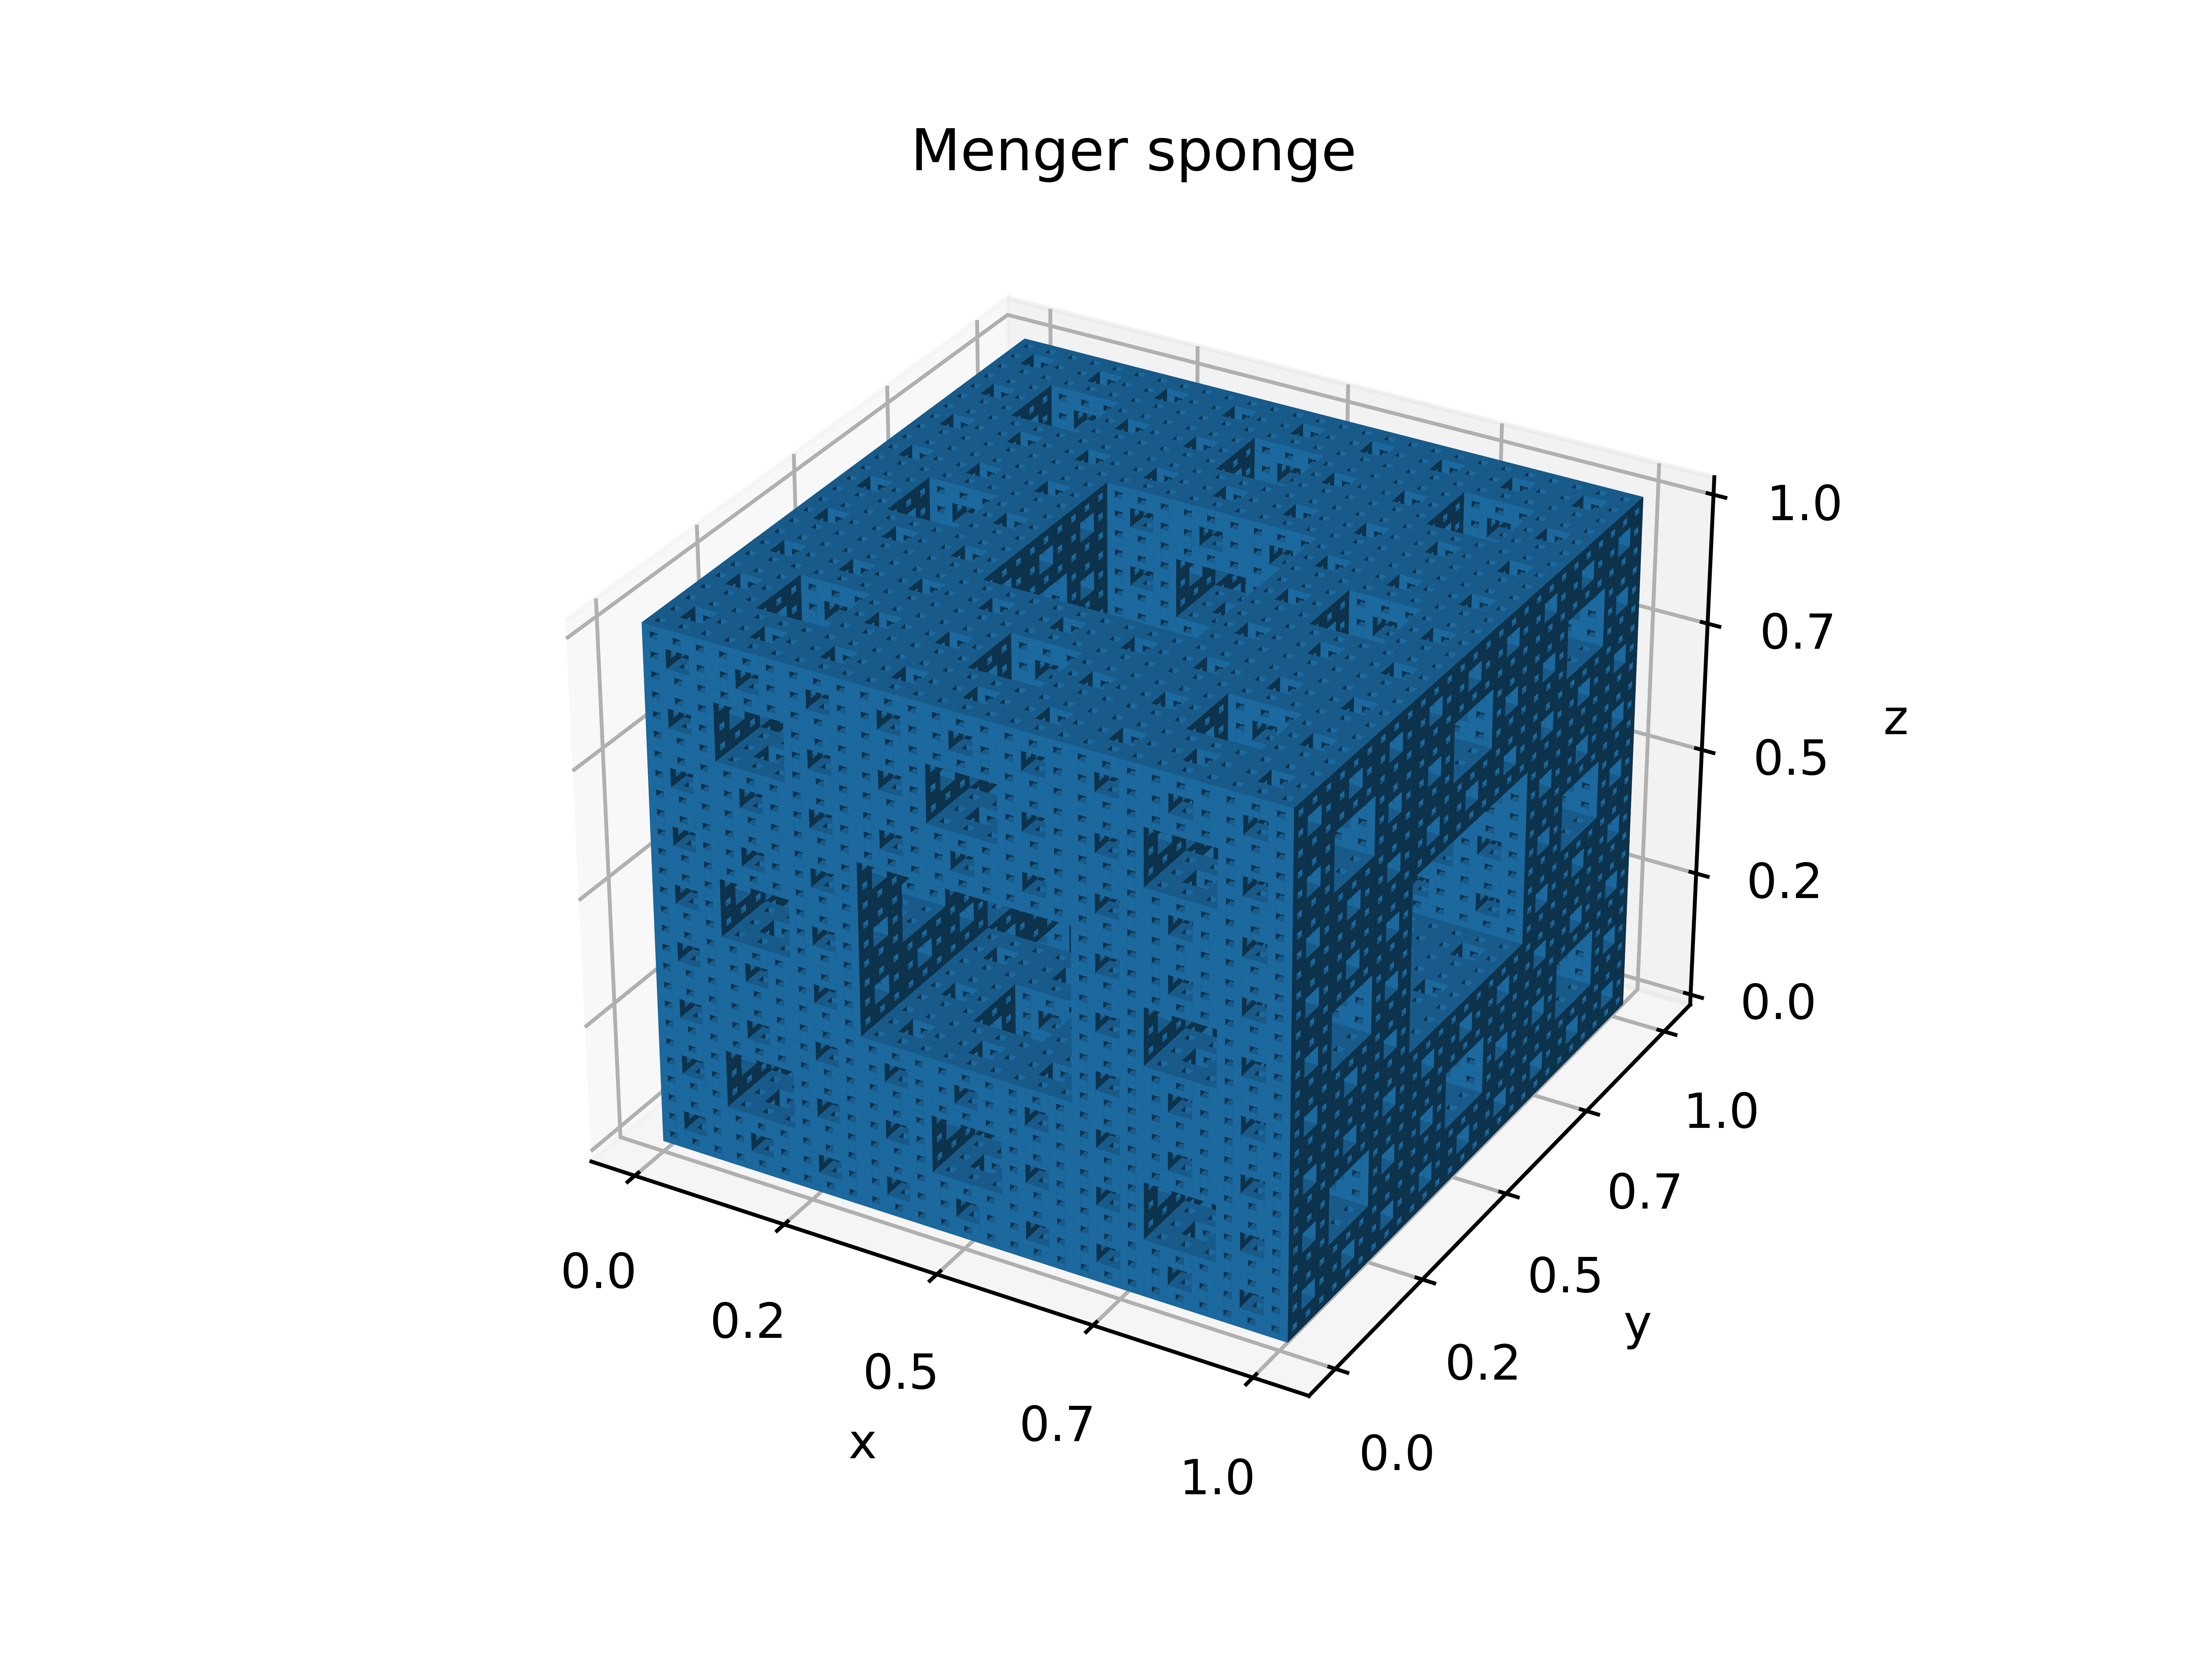
\includegraphics[width=9cm]{FA20/images/fractals/menger-3-l4-min.png}
    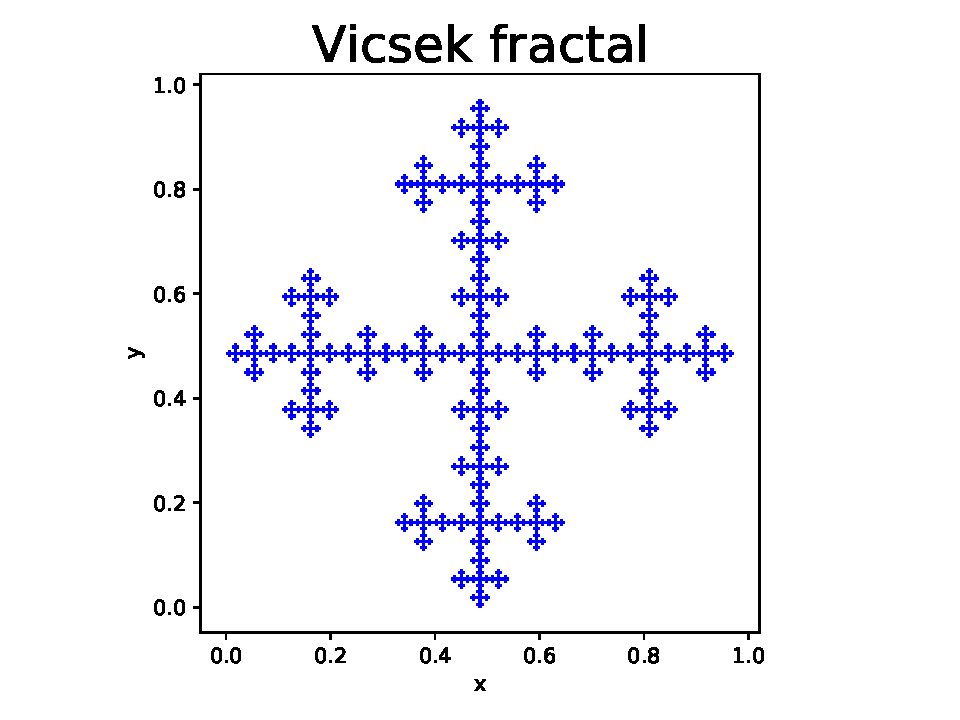
\includegraphics[width=9cm]{FA20/images/fractals/vicsek-l5.pdf}
    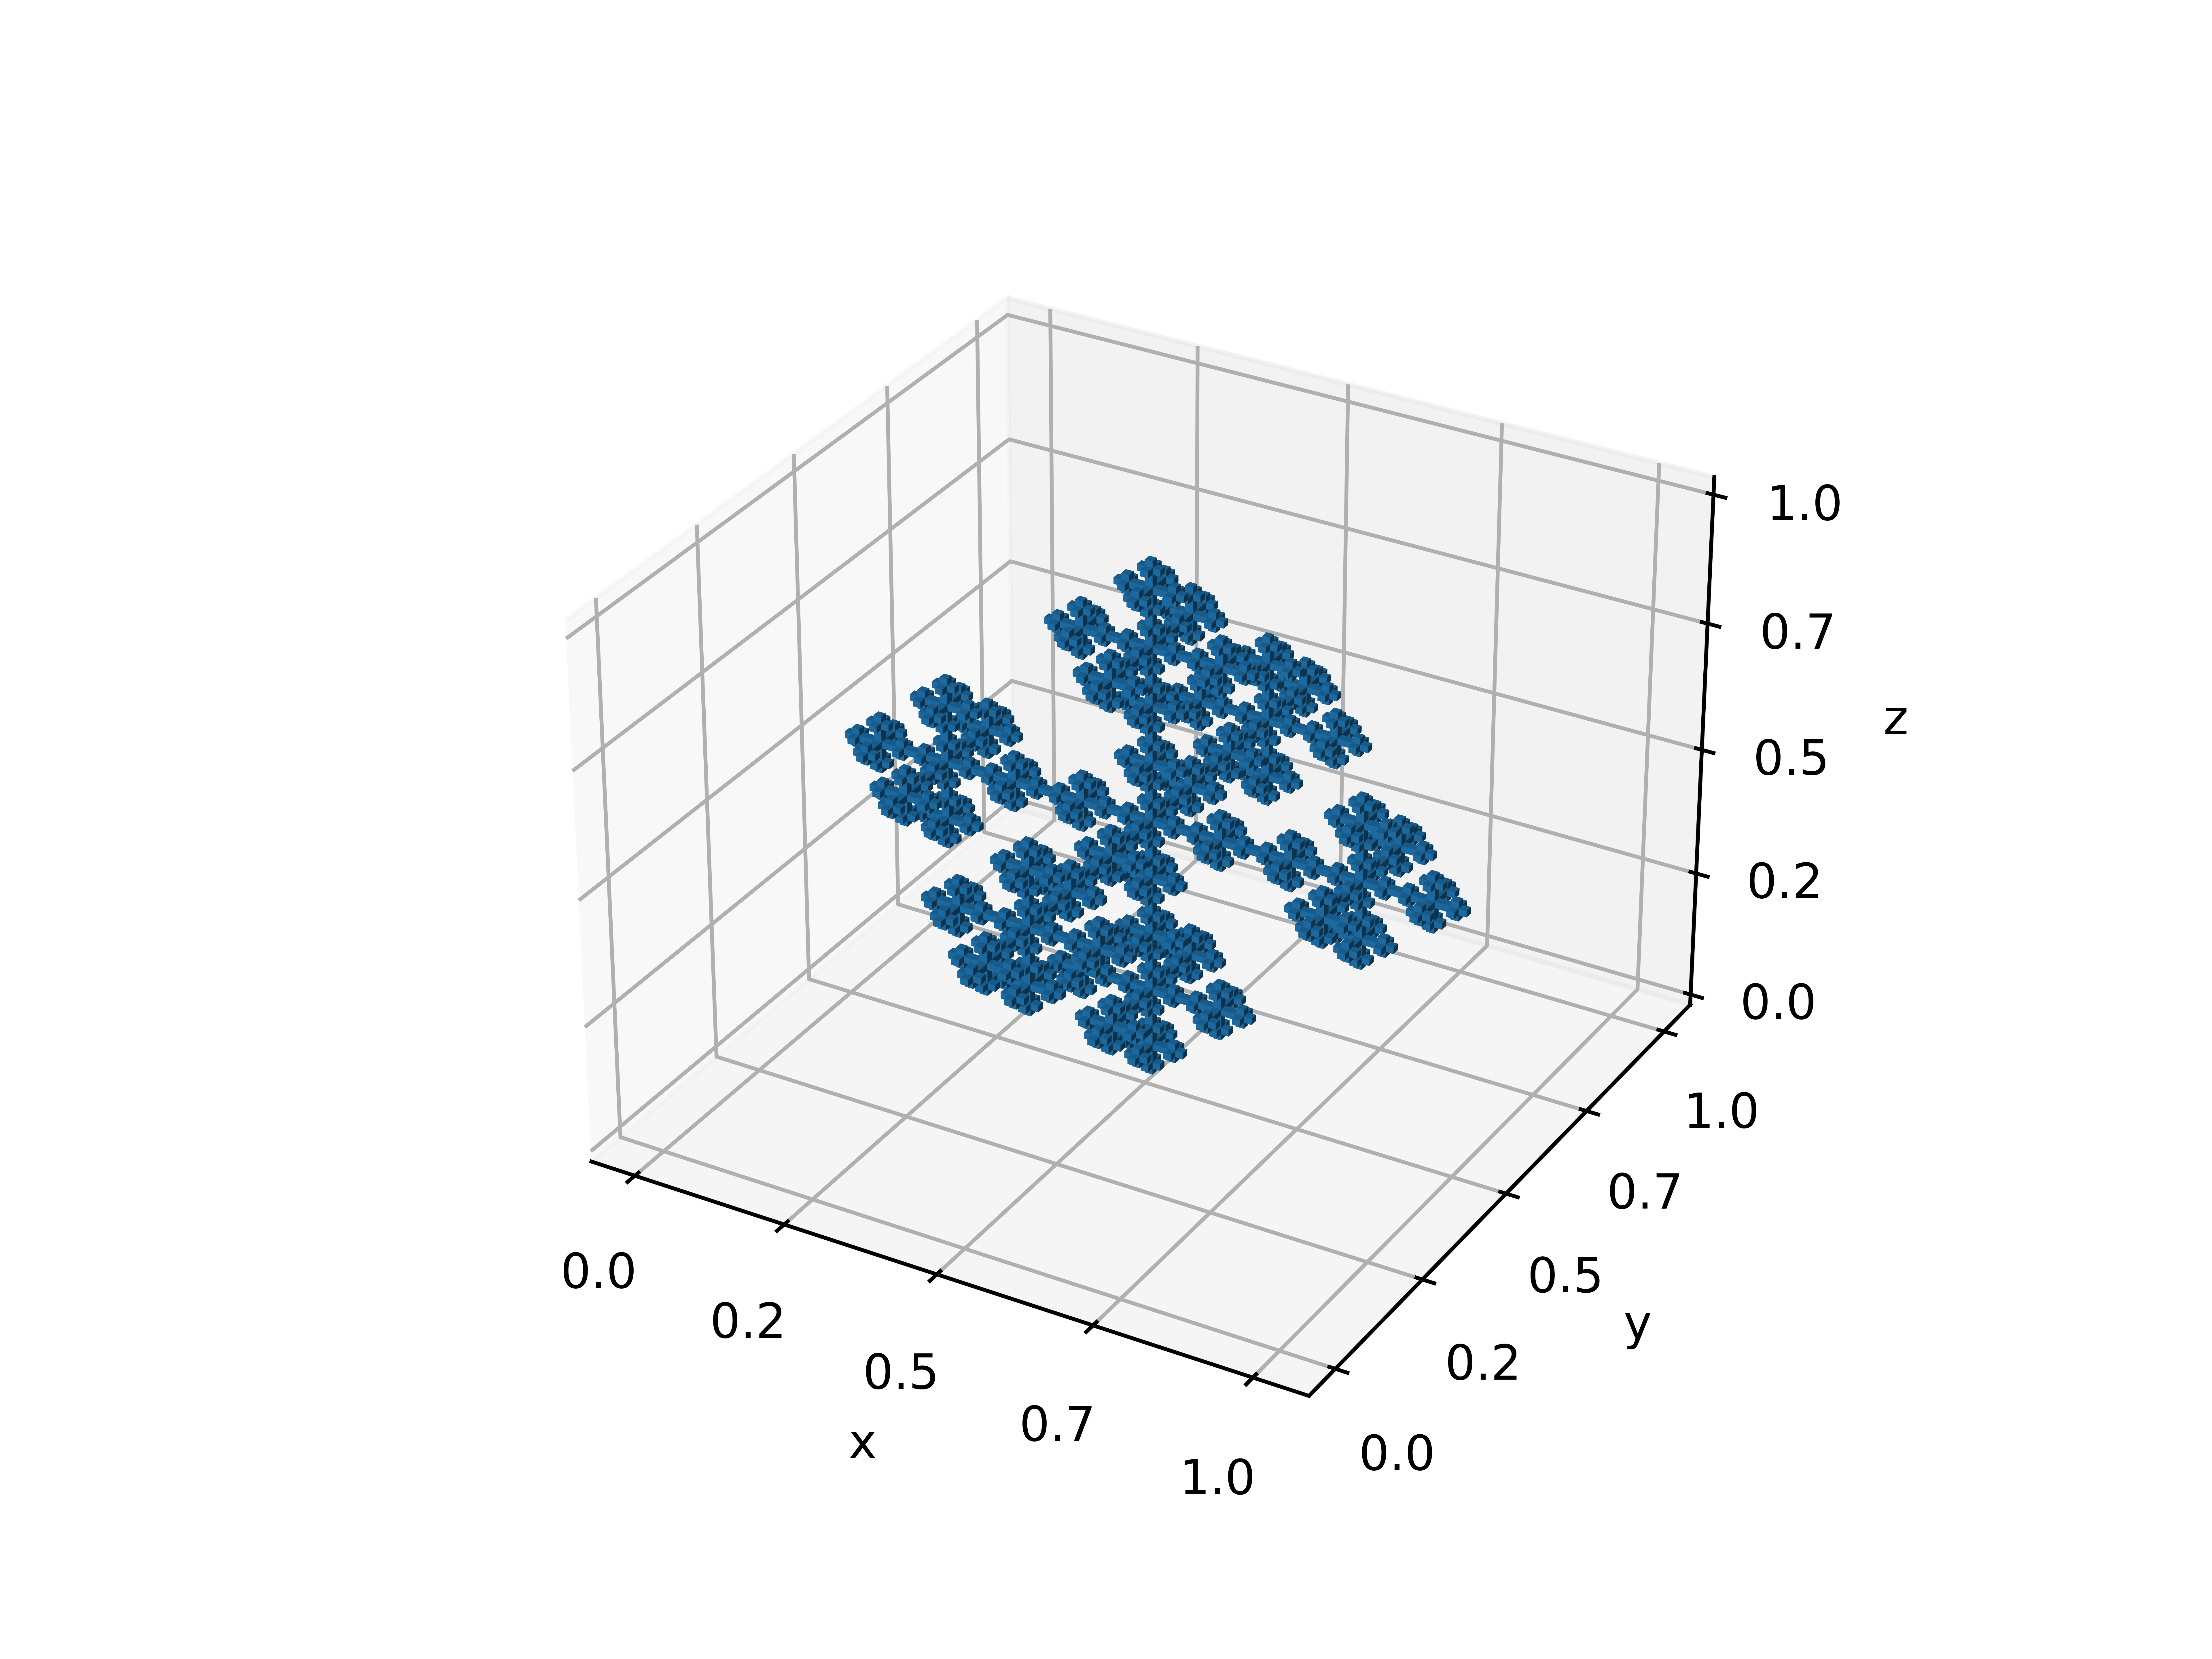
\includegraphics[width=10.5cm]{FA20/images/fractals/vicsek-3d-l4-min.png}
\end{center}
    
\begin{itemize}
        \item By adding a time variable to the automata, we can draw space-filling curves like Hilbert curve and Peano curve:
\end{itemize}
    
\begin{center}
    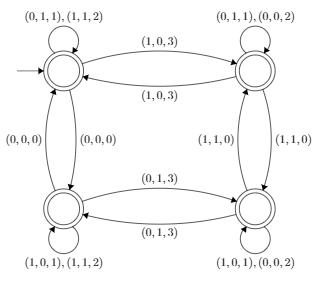
\includegraphics[width=7.5cm]{FA20/images/fractals/hilbert-automata.png}
    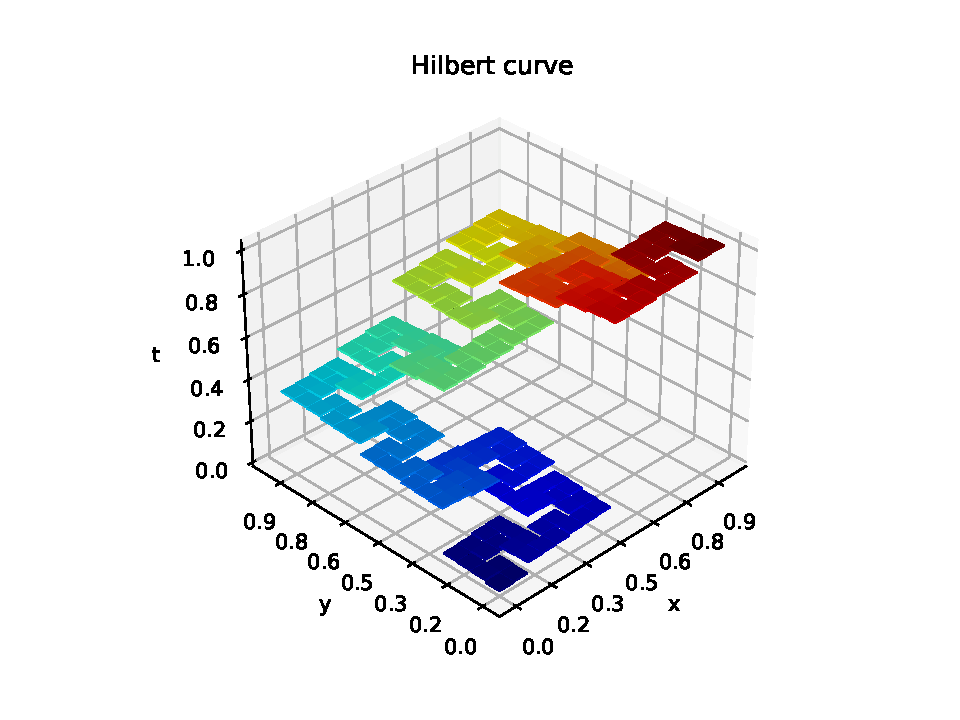
\includegraphics[width=7.5cm]{FA20/images/fractals/hilbert-1.pdf}
    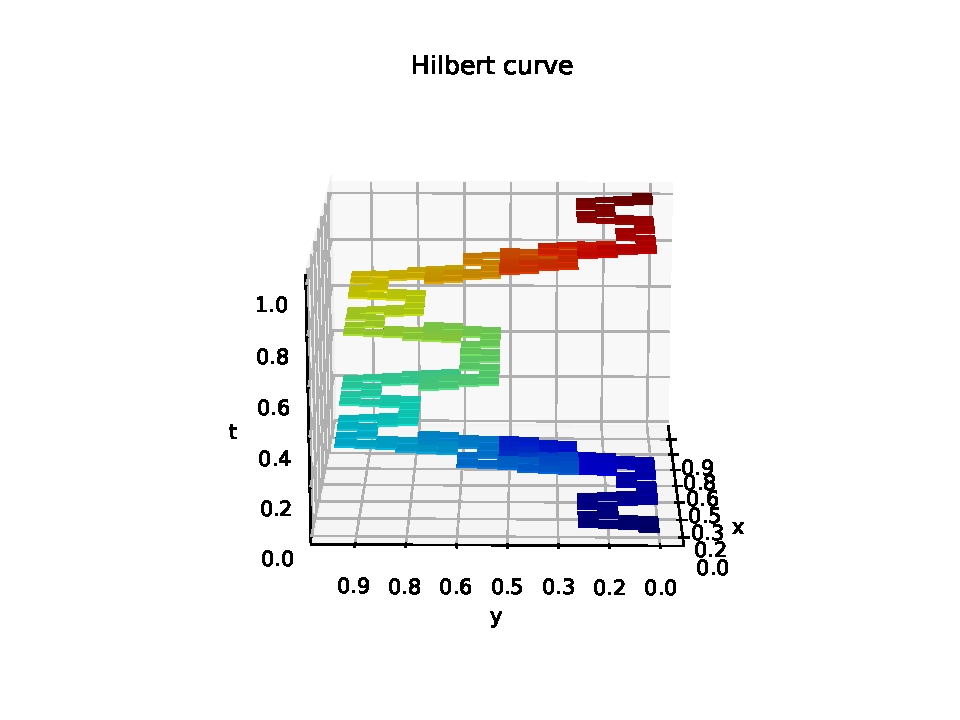
\includegraphics[width=7.5cm]{FA20/images/fractals/hilbert-2.pdf}
    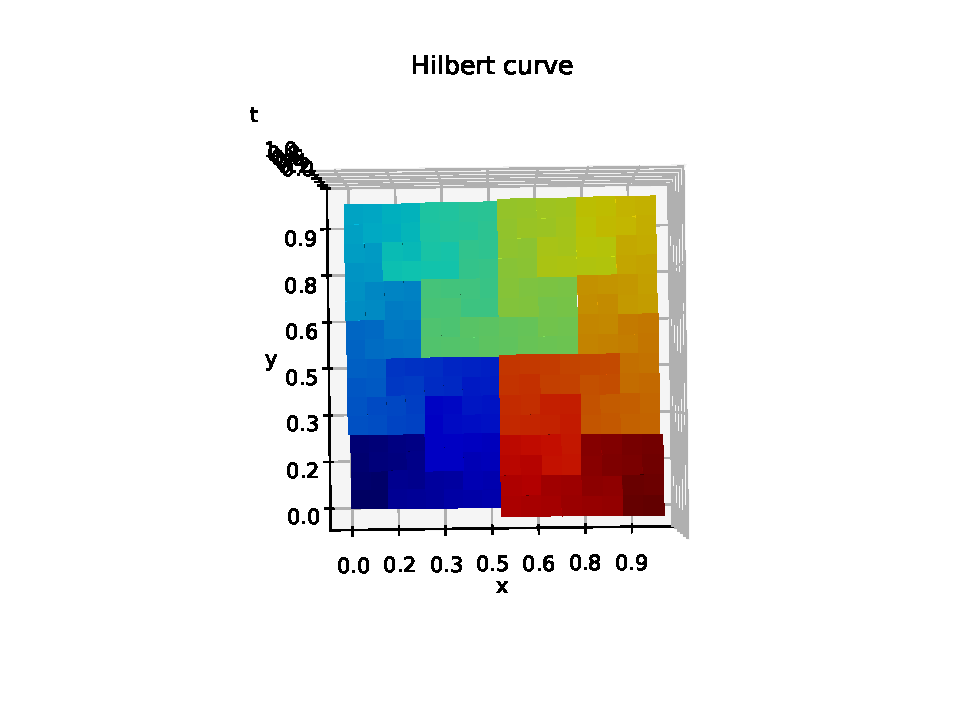
\includegraphics[width=7.5cm]{FA20/images/fractals/hilbert-3.pdf} \\
    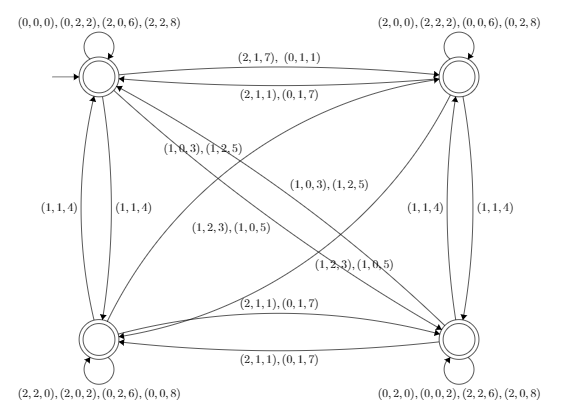
\includegraphics[width=9cm]{FA20/images/fractals/peano-automata.png}
    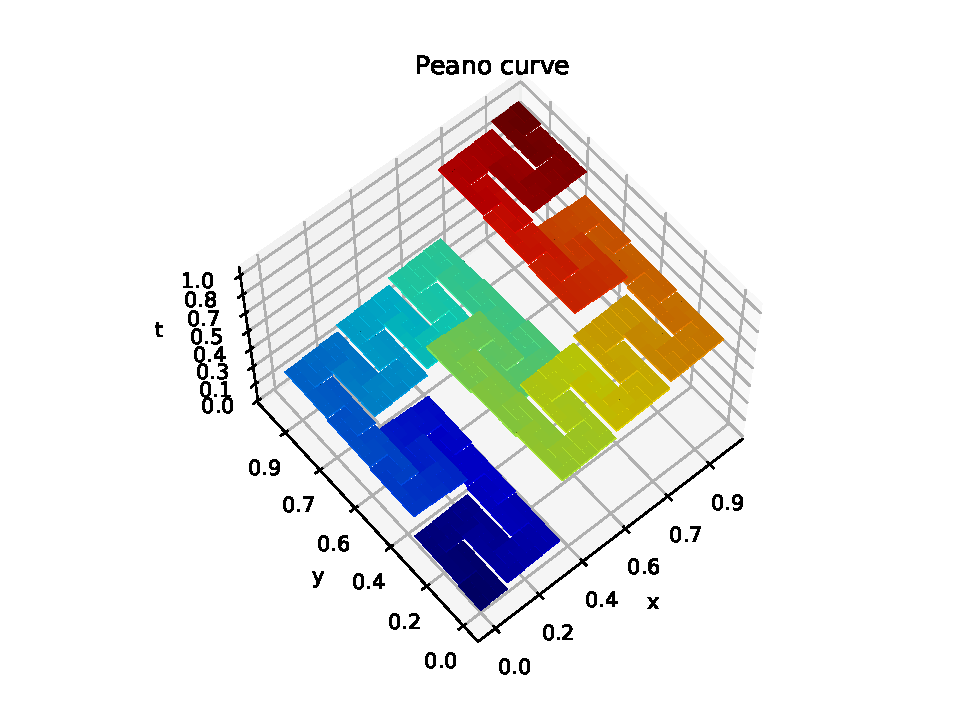
\includegraphics[width=7.5cm]{FA20/images/fractals/peano-1.pdf}
    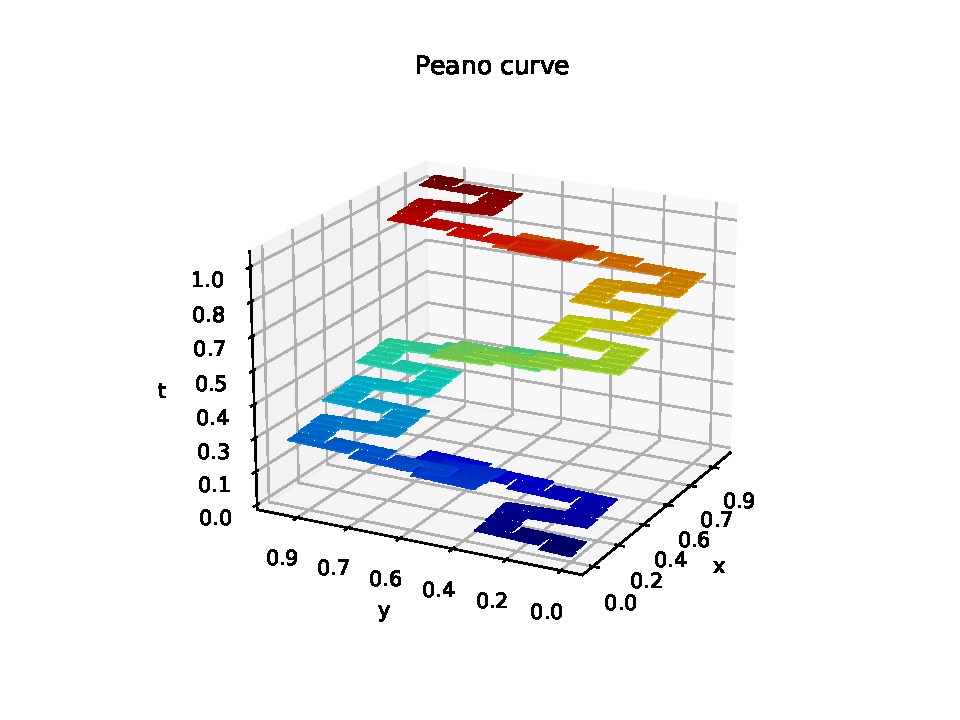
\includegraphics[width=7.5cm]{FA20/images/fractals/peano-2.pdf}
    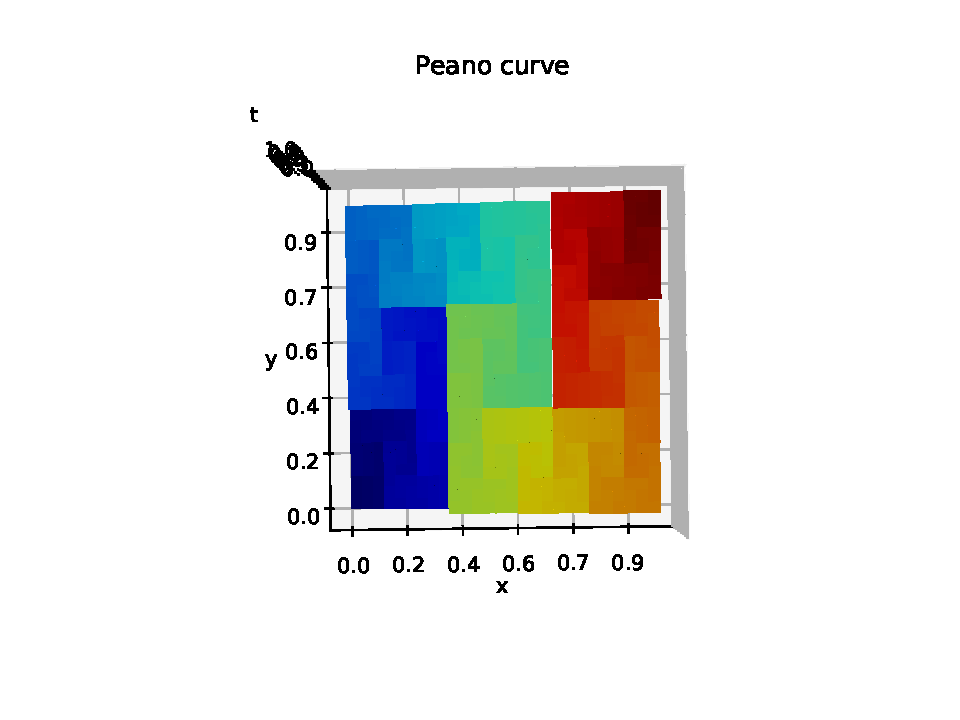
\includegraphics[width=7.5cm]{FA20/images/fractals/peano-3.pdf} \\
\end{center}    
    
\section*{Future Work}
In the future we plan to continue to develop Pecan and explore other extensions to Pecan.

% \vspace*{-10pt}  %change to -10
% \section*{References}

% {\footnotesize [1] Khoussainov, Bakhadyr.Nerode, Anil. (2001) \emph{Automata Theory and its Applications}, MA : Birkh\"auser Boston}

% {\footnotesize [2] Hamoon Mousavi. \emph{Automatic Theorem Proving in Walnut}. In: CoRR abs/1603.06017 (2016).
% arXiv: 1603.06017. url: http://arxiv.org/abs/1603.06017.}

% {\footnotesize [3] Du, Chen Fei. Mousavi, Hammoon. Schaeffer, Luke and Shallit, Jeffrey. (2014) \emph{Decision Algorithms for Fibonacci-Automatic Words, with Applications to Pattern Avoidance}
% }

% {\footnotesize [4] Hieronymi, P., \& Terry Jr, A. (2018). \emph{Ostrowski Numeration Systems, Addition, and Finite Automata}. Notre Dame Journal of Formal Logic, 59(2), 215-232.
% }

{
\footnotesize
\bibliographystyle{unsrt}
\bibliography{biblio}

[2] Khoussainov, Bakhadyr.Nerode, Anil. (2001) \emph{Automata Theory and its Applications}, MA : Birkh\"auser Boston

[3] Hamoon Mousavi. \emph{Automatic Theorem Proving in Walnut}. In: CoRR abs/1603.06017 (2016).

[4] Philipp Hieronymi, Danny Nguyen, Igor Pak. (2019) \emph{Presburger Arithmetic with algebraic scalar mutliplications.} arXiv:1805.03624.
}

\vspace*{10mm} %This will change to -5
\emph{Support for this project was provided by the Illinois Geometry Lab and the Department of Mathematics at the University of Illinois at Urbana-Champaign. This project was partially supported by NSF grant DMS-1654725. Any opinions, findings, and conclusions or recommendations expressed in this material are those of the author(s) and do not necessarily reflect the views of the National Science Foundation.}
\end{multicols}

\end{document}
